\chapter{Simulation}
\label{ch:Simulation}

\section{Simulation of pp collisions}
\subsection{MC Generators Used for LHC Physics}
\subsection{Detector Simulation}
\subsection{Showering in the Detector}
\section{Object Reconstruction}
\subsection{Electrons}
\subsection{Photons}
\subsection{Jets}
\subsubsection{B-Jets}
\label{sec:bjetReco}
\subsection{Muons}
\subsection{Creation of FCNC Signal Events}
\subsubsection{MadGraph5 amc@NLO}
Comparison of kinematics between standard ttbar events
ATLAS Production of these events
TopQ1 Slimming/Skimming





%
%%%%%%%%%%%%%%%%%%%%%%%%%%%%%%%%%%%%%%%%%%%%%%%
%%%%%%%%%%%%                                                                                                   %%%%%%%% 
%%%%%%%%%%%%                           BEN                                                                  %%%%%%%% 
%%%%%%%%%%%%                                                                                                   %%%%%%%% 
%%%%%%%%%%%%%%%%%%%%%%%%%%%%%%%%%%%%%%%%%%%%%%%
%
%
%\chapter{The Strong Force and Jets}
%\label{ch:Jets}
%
%The cross-section for the collision of two hadrons can be written as
%\begin{equation}
%d\sigma_{AB\rightarrow J+X} = \sum_{a,b}^{}\int dx_a dx_b f_{a/A}(x_a, \mu_F^2) f_{b/B}(x_b, \mu_F^2) \times d\hat{\sigma}_{ab\rightarrow J+X} (\alpha_s(\mu^2_R),Q^2)
%\end{equation}
%where $A$ and $B$ are the incoming hadrons (in the case of the LHC, protons), $J+X$ are an observable plus any other particle, such as two jets, or a jet plus some invisible particle, $a$ and $b$ are the types of partons (the six quark flavors and the gluon), $d\hat{\sigma}_{ab\rightarrow X} (\alpha_s(\mu^2_R),\mu^2)$ is the cross-section for the collision of the two partons $a$ and $b$ to produce $X$, which can be calculated directly from theory and depends on the the scale of the interaction, $\mu$, and strong QCD coupling, $\alpha_s$, measured at renormalization scale $\mu^2_R$.  This formula is approximate and has corrections of surpressed by a factor of 1~GeV/$Q$.  For the energies probed in this analysis, with jets on the order of 1~TeV, these corrections are very small.
%
%The renormalization scale is used to absorb the ultraviolet divergences which come from the higher-order diagrams of the process, imposing a cutoff on the energy in exchange for making $\alpha_s$ depend on this scale.\cite{StrongCoupling}  This is the origin of the running coupling of the strong interaction, where the strength of the coupling decreases as the energy of the process increases.  Similarly, the parton distribution functions discussed in the next section depend on the choice of factorization scale.  
%
%While the choice of scale is arbitrary and should not have an effect on the cross-section, this is only true if one is able to expand out to infinite accuracy, as $\hat{\sigma}$ has an expansion in powers of $\alpha_s$.  With a good choice in scale, good accuracy to the full expansion can be obtained with only a few terms in the series.   With the choice of renormalization and factorization scales close to the scale of the given process such that $\mu^2_R = \mu_F^2 \simeq Q^2$, the cross-section can be characterized by only the energy scale of the interaction and is well described by the expansion.  This choice of scales is used for the remainder of this chapter.
%
%The final factors, $f_{a/A}(x_a, Q^2)$, are the parton distribution functions, or PDFs.  The PDFs represent the probability density for a parton of type $a$ to carry a fraction $x_a$ of the total momentum of the hadron.  The total cross section for the process is then the sum over all of the types of partons from the two incoming hadrons.
%
%
%
%\section{Parton Distribution Functions}
%
%Since the proton is a composite particle, its overall momentum is equivalent to the sum of the momenta of its constituents.  Given the large momenta of accelerated protons in the LHC for Run 2, this is equivalent to saying that the total energy of the proton (6.5\,TeV for Run 2) is divided up between the partons that comprise the proton.
%
%PDFs can not be calculated from theory but instead must be taken directly from data, much of which comes from deep inelastic scattering experiments from electron-proton colliders, in addition to Drell-Yan and inclusive jet production measurements from proton-proton colliders, including results from Run 1 of the LHC.  Once the PDF at a given energy transfer $Q$ is known, the PDF can be evolved to other energies using the Dokshitzer-Gribov-Lipatov-Altarelli-Parisi~(DGLAP) equations.\cite{DGLAP1,DGLAP2,DGLAP3}  Examples of the proton PDF at two different energy scales are shown in Figure~\ref{fig:CT14PDFs}.  
%
%While one would naively expect the momentum to be roughly split between the two up quarks and one down quark, this is not the case.  Rather, a sizeable portion of the momentum is carried by gluons which constantly radiate from and are reabsorbed by the valence quarks.  These gluons can also fluctuate into quark-antiquark pairs, referred to as $sea~quarks$.  At higher $Q$, shorter distance scales are probed, meaning larger fluctuations are accessible, and thus larger amounts of momentum are carried by the gluons and sea quarks rather than just by the valence quarks.
%
%\begin{figure}[h!]
%	\centering
%	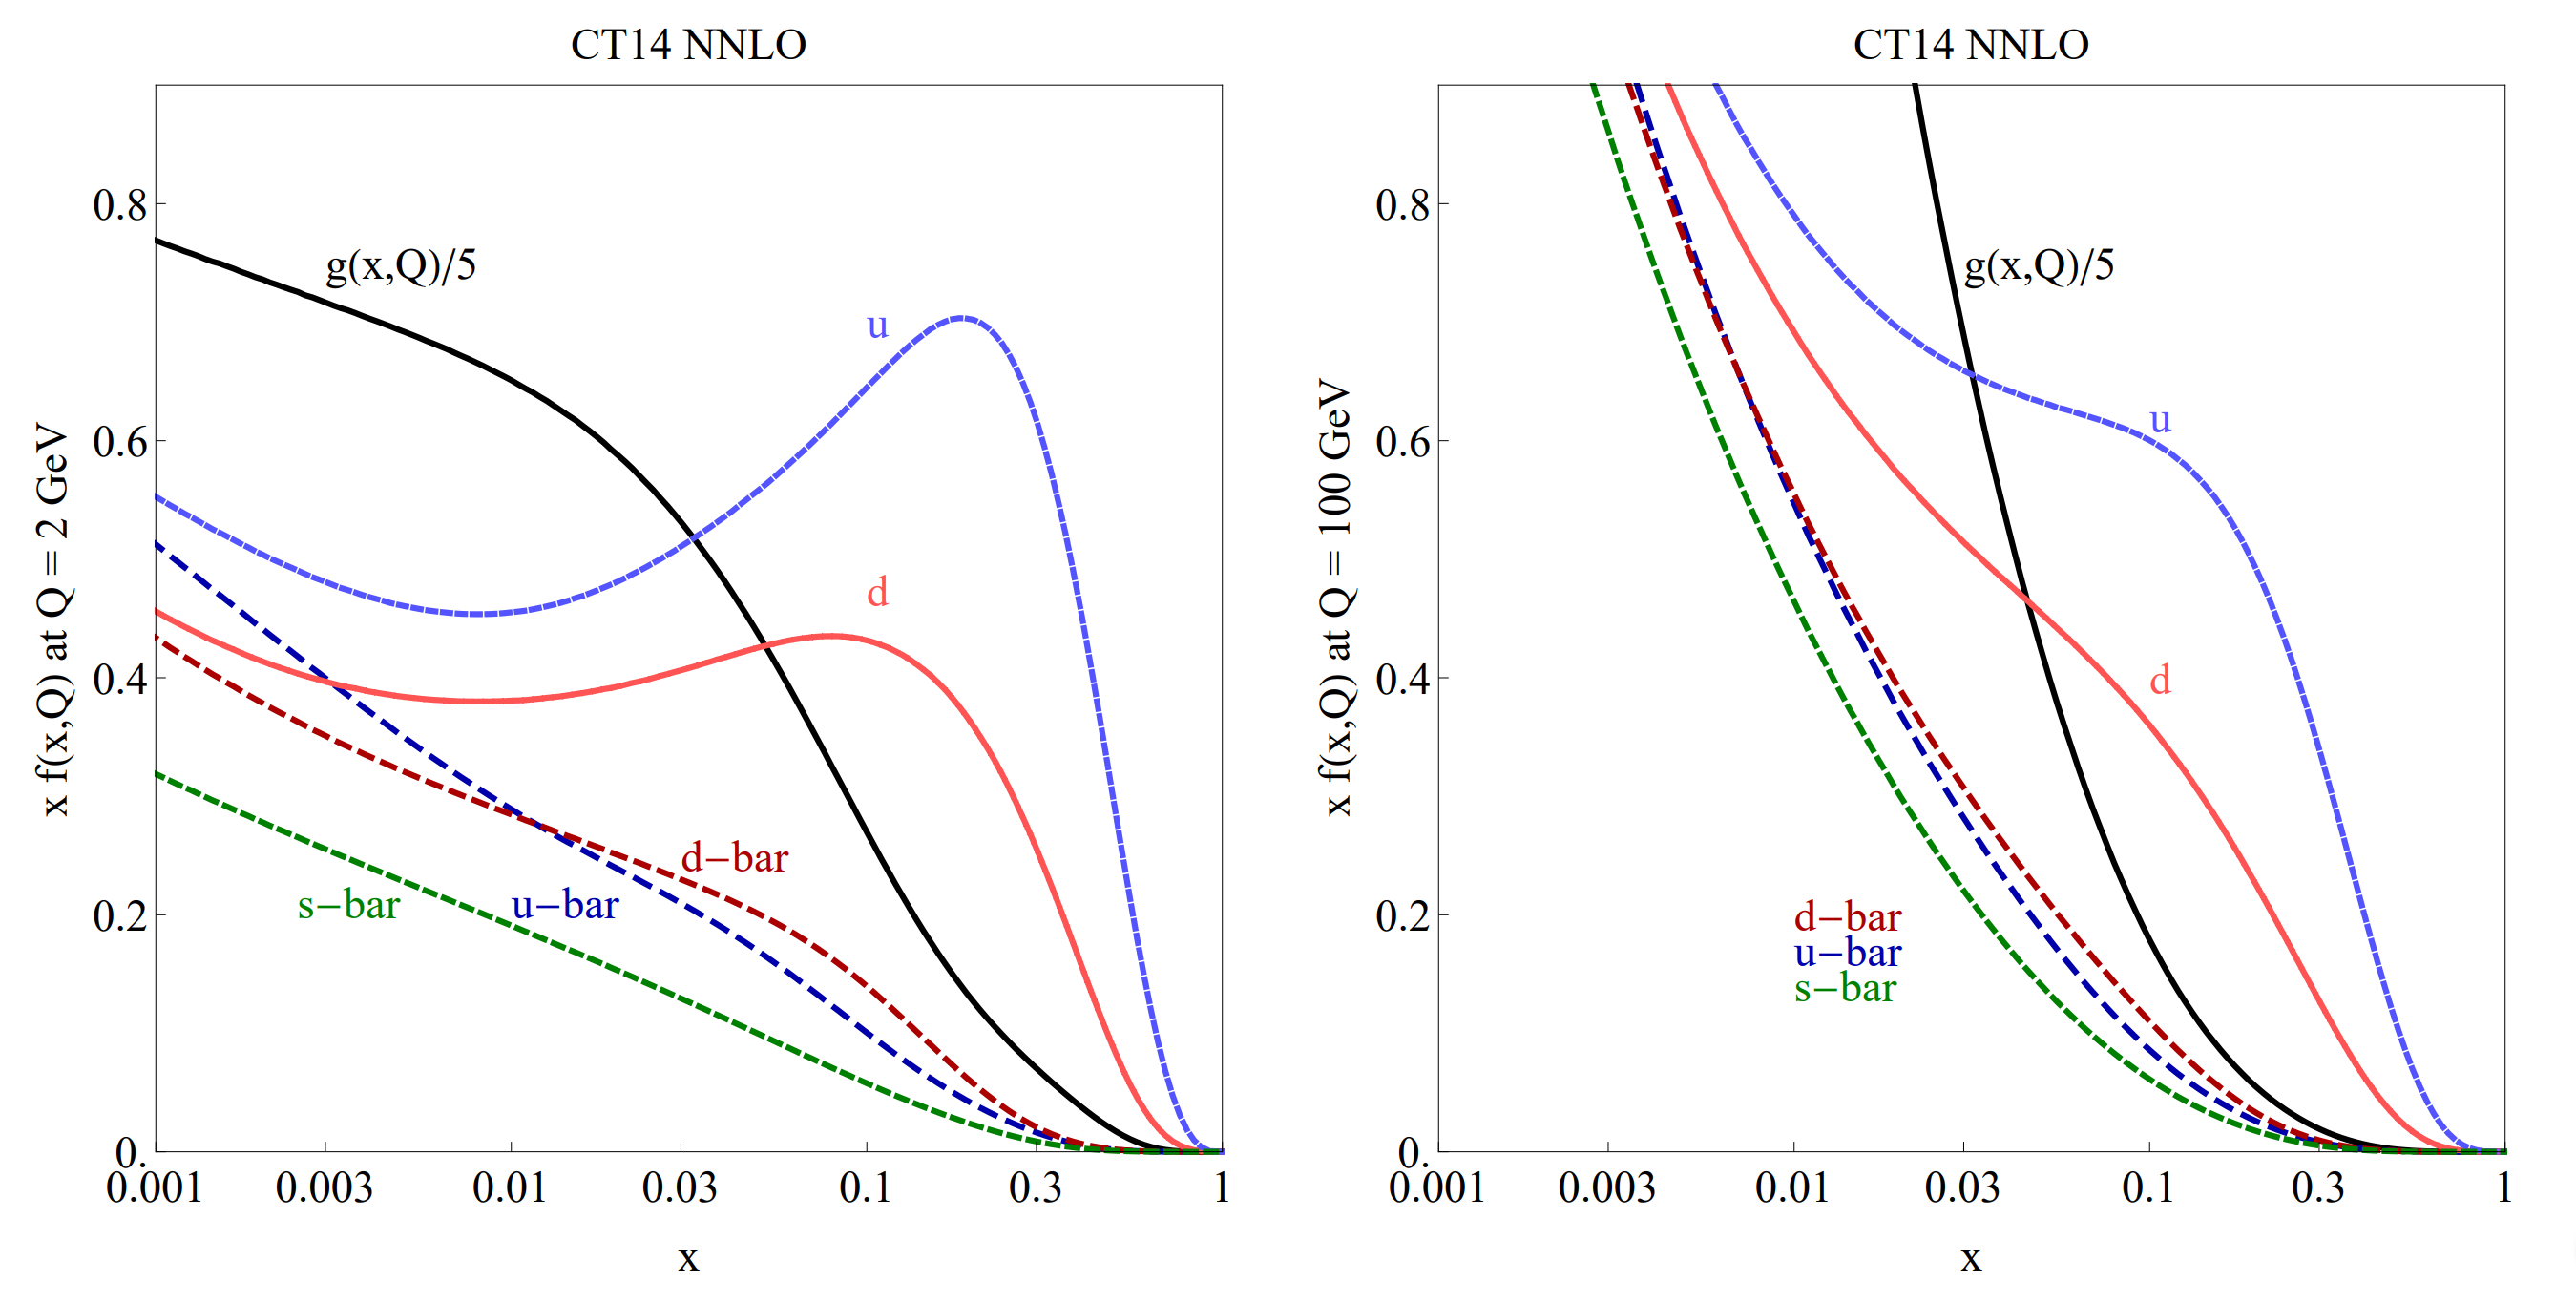
\includegraphics[width=\columnwidth]{figures/Jets/CT14PDFs.png}
%	\caption{The measurement of parton distribution functions (PDFs) from the CTEQ collaboration. PDFs are shown at Q = 2\,GeV and Q = 100\,GeV for $u, \bar{u}, d, \bar{d}, s = \bar{s}$, and $g$.  The full results can be seen in Ref.~\cite{CT14PDF}.
%	}
%	\label{fig:CT14PDFs}
%\end{figure}
%
%The high-mass dijet search relies on interactions at high-$Q$ and partons at very high-$x$ in the PDF, where $x$ is the fraction of the total proton momentum carried by a given parton.  However, while the valence quarks are the most common at high-$x$, there are no quark-quark vertices in the standard model, only quark-antiquark and (anti)quark-gluon ones.  The t-channel quark-quark scattering is then the dominant background in a dijet search over s-channel processes from both Standard Model QCD and any possible new resonances.  Figure~\ref{fig:Feynman} shows a comparison of these two channels.  This background is suppressed in the analysis by imposing a maximum difference in rapidities between the two leading jets, as t-channel processes peak at very high rapidity near the beam line.  In the limit of massless quarks (a safe assumption given the energies probed by the high-mass dijet search), the Mandlestam variables can be written as:
%
%\begin{equation}
%\hat{s} = (p_1+p_2)^2 = \mjj^2
%\end{equation}
%\begin{equation}
%\hat{t} = -\frac{1}{2}\hat{s}(1-cos~\theta^*)
%\end{equation}
%where $\theta^*$ is the polar angle from the beam line to the outgoing parton in the center-of-mass frame, and \mjj~is the invariant mass of the dijet system.\cite{EllisQCD}  The matrix element for the $s$-channel process is proportional to $\hat{s}^{-1}$, while the $t$-channel process is proportional to $\hat{t}^{-1}$.  Thus, the $s$-channel production is independent of angle, while the $t$-channel mode peaks at angles close to the beam line and is minimized in the central region of the detector.
%
%\section{Anatomy of a Collision}
%
%While the Feynman diagrams for dijet production look simple, proton-proton collisions are extremely convoluted, as evidenced by Figure~\ref{fig:HadronEvent}.  In addition to the hard scatter and decays (in red), the event also contains many gluon emissions from the strongly charged particles (blue) as well as secondary interactions from the other proton constituents (purple).  These colored particles then group into colorless baryons and mesons, which in turn have their own decays (green).
%
%\begin{figure}[h!]
%	\centering
%	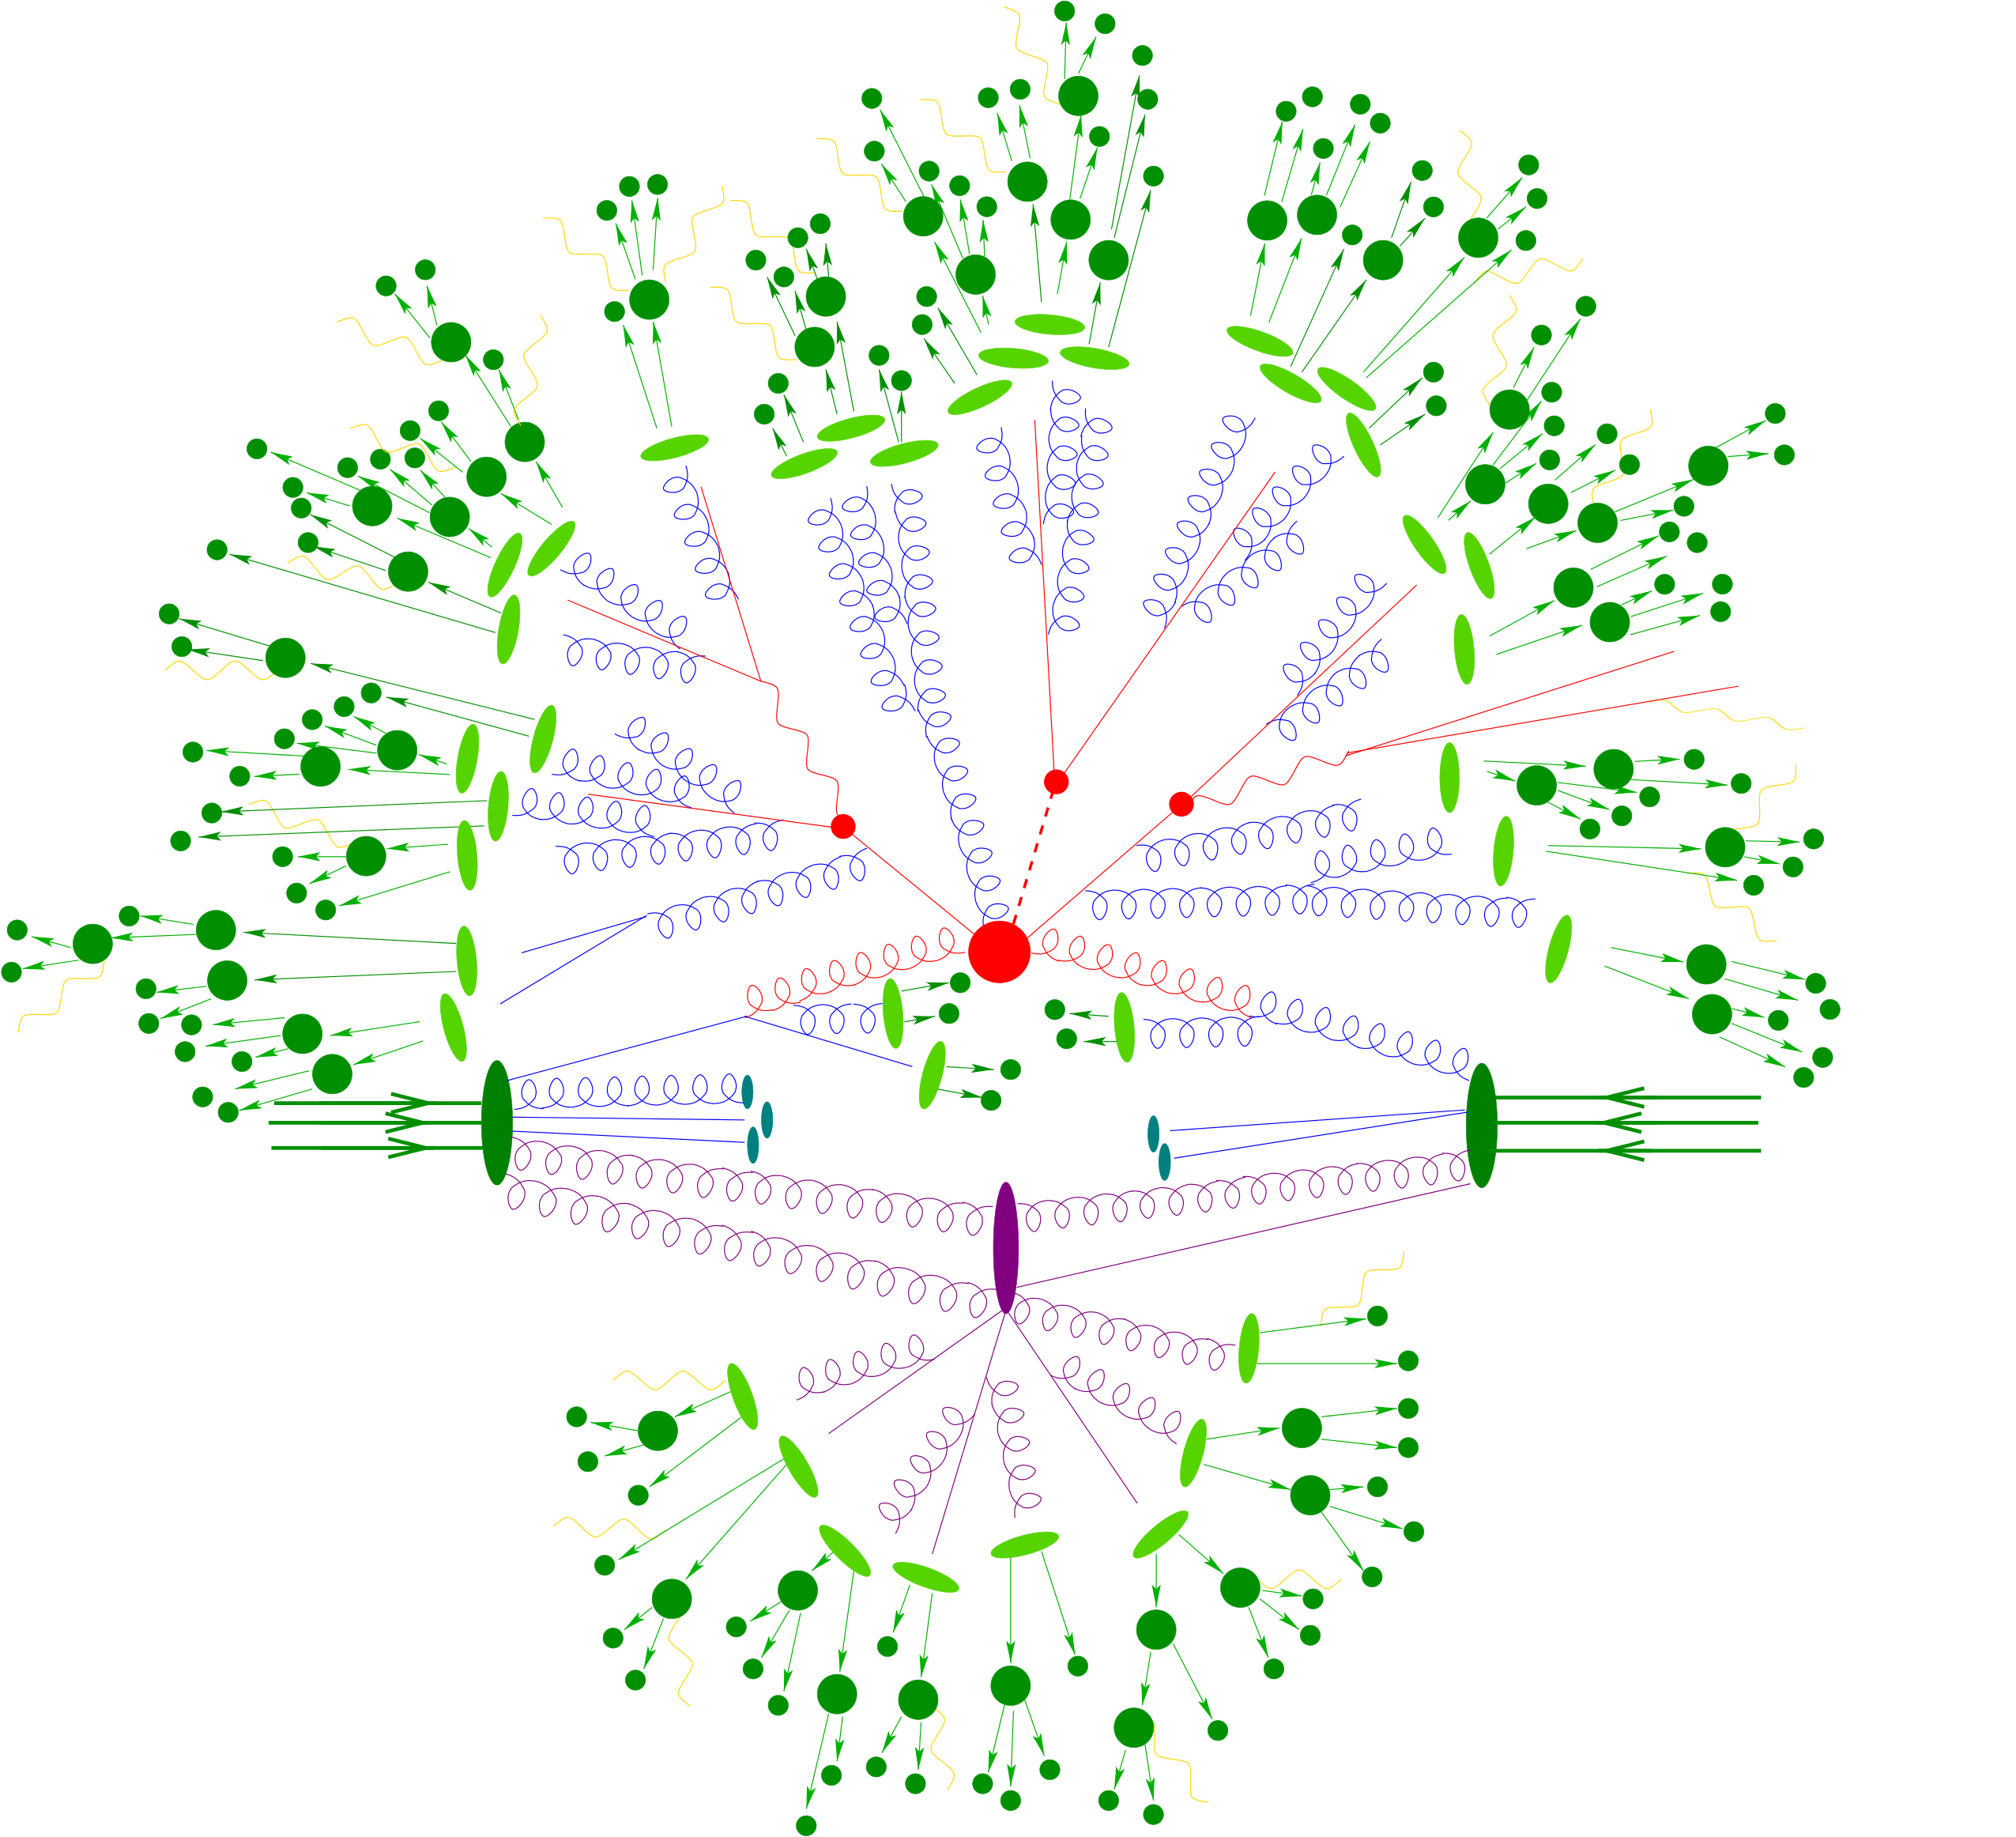
\includegraphics[width=\columnwidth]{figures/Theory/HadronEvent.jpg}
%	\caption{Simulation of a sample proton-proton collision.  The incoming partons are in blue, the underlying event interactions are in purple, the hard scattering event is in red, and the hadronization processes are shown in green.  Image from~\cite{Sherpa}.
%	}
%	\label{fig:HadronEvent}
%\end{figure}
%
%\subsection{Hard Scatter and Parton Showering}
%
%The hard scatter is the interaction of interest in an event, with two partons interacting and producing the high transverse energy final state of interest.  The Feynman diagrams for a collision correspond to the hard scatter, such as the $gg\rightarrow tth$ process shown in Figure~\ref{fig:HadronEvent}.  Here, the Higgs decays into a pair of quarks, and the two top quarks decay to $bW$, with one $W$ decaying hadronically and the other leptonically, as shown in red.  In addition, the free partons from the hard process undergo parton showering, whereby a quark or gluon can radiate a nearly-collinear gluon which carries away some portion of its momentum.  In addition, a gluon can produce a quark-antiquark pair.  This process continues until the splittings reach low enough virtuality that can no longer be described perturbatively, beyond which point confinement takes effect and the partons $hadronize$ into the colorless particles which can be observed by the detector.
%
%\subsection{Pileup and Underlying Event}
%
%The underlying event, shown in purple in Figure~\ref{fig:HadronEvent}, is the interaction of the remaining partons in the $pp$ collision which did not participate in the hard scatter.  These remnants can interact with each other and produce softer interactions which then overlay with the products from the hard scatter of interest.
%
%ATLAS produces collisions by colliding bunches with $\sim10^{11}$ protons each, and as such a variable number of collisions occur each bunch crossing.  For a typical data event taken in 2016, a single hard scatter event was also accompanied by some two dozen other softer scatters, often referred to as pileup.  The distribution of the number of pileup interactions can be seen in Figure~\ref{fig:LumiPileup}.  Pileup takes two forms: in-time pileup which produces particles which appear simultaneously in the detector with the hard scatter products, and out-of-time pileup where particles from previous bunch crossings are still traveling through the detector.
%
%The effect of both the underlying event and a single pileup event is roughly the same: it adds additional calorimeter noise and physics objects which make it more difficult to pick out only the hard scatter products.  An example event is shown in Figure~\ref{fig:PileupEvent} where a single $Z\rightarrow\mu\mu$ event with 24 pileup interactions is shown.  All of the energy deposited in the calorimeter, with the exception of the small amount along the path of the muons, comes from the underlying event and pileup interactions.  While this can have a large effect on searches using lower-momentum objects or missing transverse energy, the high-mass dijet search is relatively insensitive to their effects owing to the large discrepancy in energy scales between typical pileup interactions and the hard scatters of interest.
%
%\begin{figure}[h!]
%	\centering
%	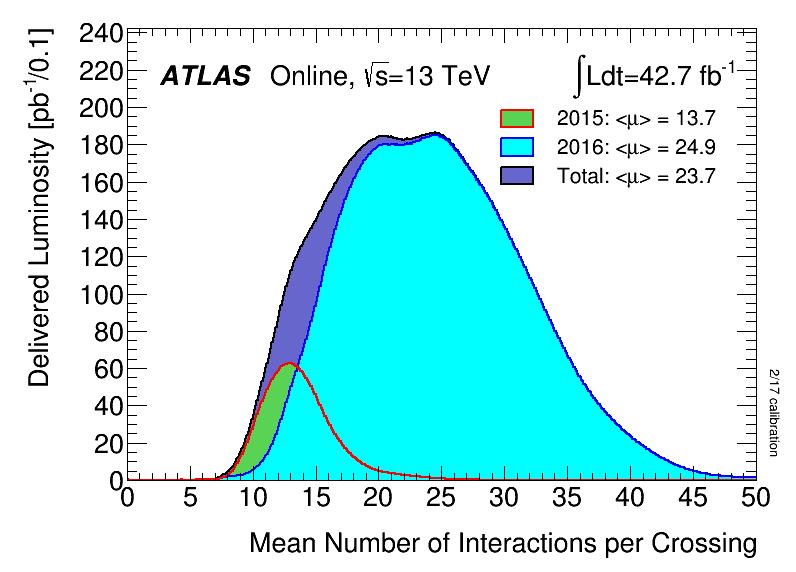
\includegraphics[width=0.5\columnwidth]{figures/Jets/LumiPileup.png}
%	\caption{Luminosity-weighted distribution of the mean number of interactions per crossing for the 2015 and 2016 datasets.
%	}
%	\label{fig:LumiPileup}
%\end{figure}
%
%\begin{figure}[h!]
%	\centering
%	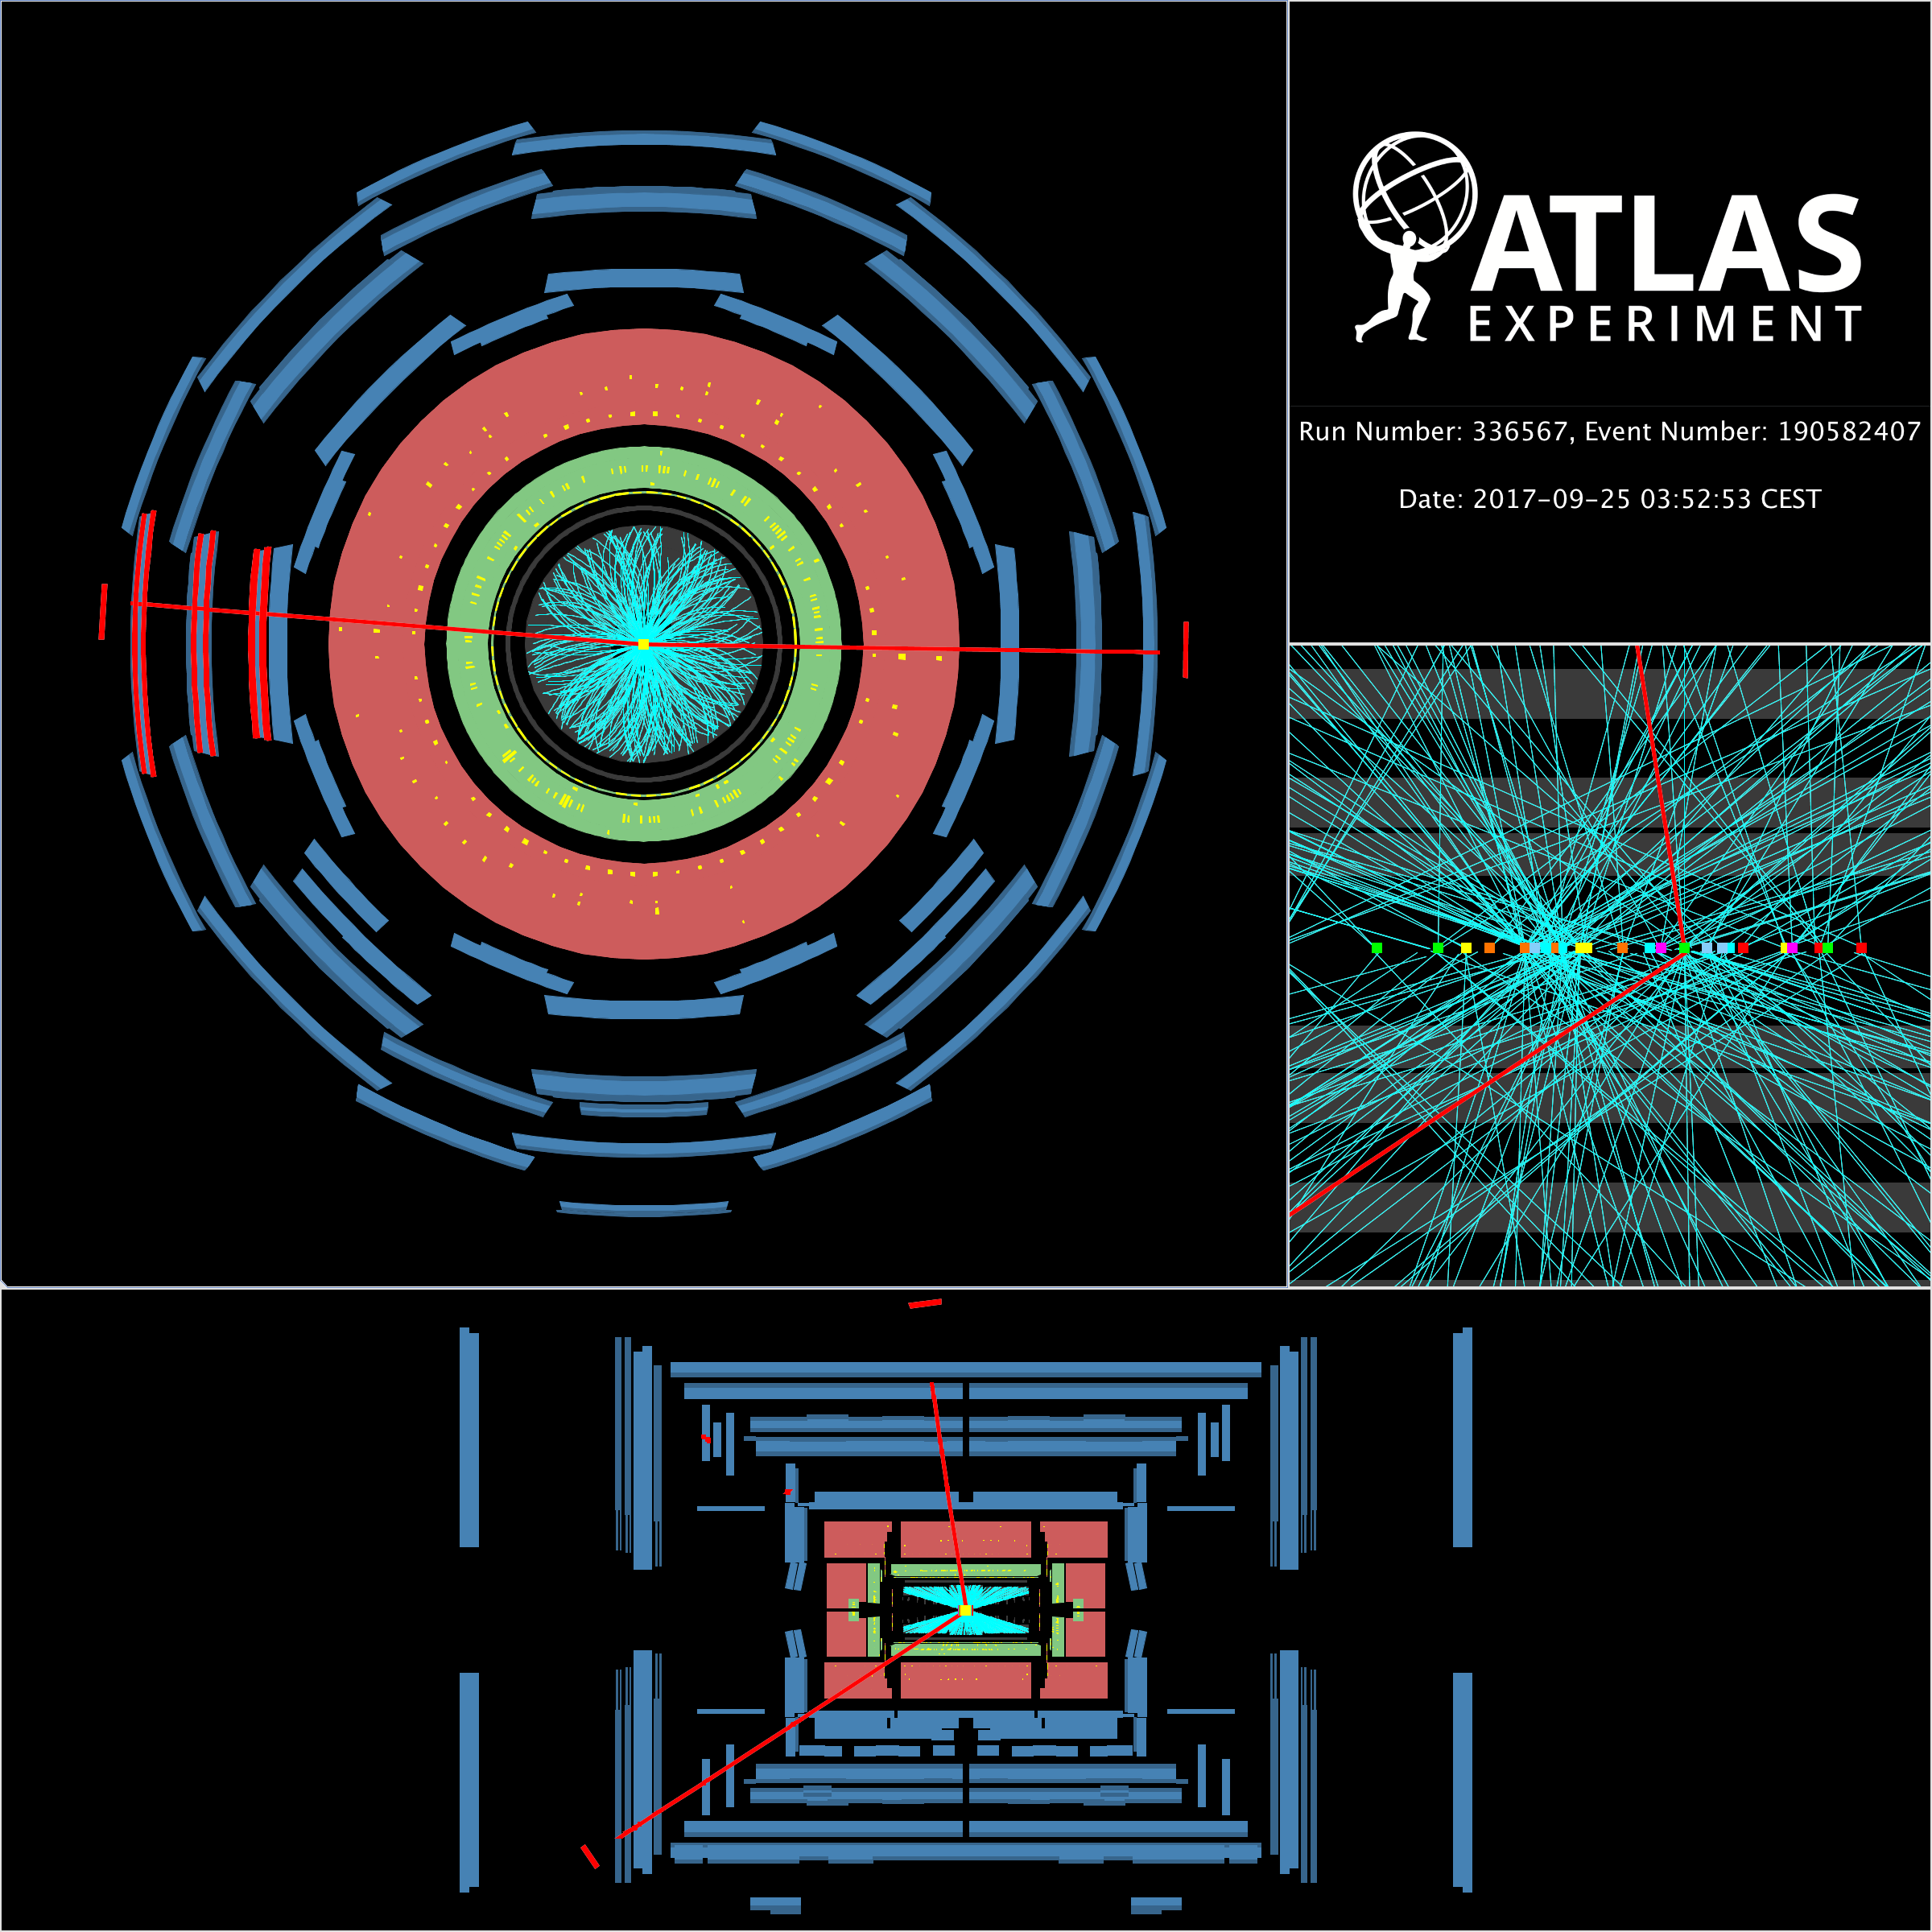
\includegraphics[width=\columnwidth]{figures/Jets/PileupEvent.png}
%	\caption{Event display of a $Z\rightarrow\mu\mu$ event with 24 other reconstructed vertices from pileup interactions.  The paths of the two muons are shown in red, while the blue lines are tracks with $\pt >$ 500\,MeV 
%	}
%	\label{fig:PileupEvent}
%\end{figure}
%
%\subsection{Hadronization}
%
%As the partons and their showering products in the collision move to longer distances, the process of hadronization occurs whereby the colored partons are formed into colorless baryons and mesons which will then decay into the final state particles which are seen by the detector.  An exact description of hadronization in QCD is not known, but there are several models used in Monte Carlo generators which work very well, including the Lund string model~\cite{LundStringModel} used in the Pythia~\cite{Pythia} generator, and the cluster model~\cite{ClusterModel} used in the Herwig~\cite{Herwig} generator.  The particular showering process used has almost no effect on the sensitivity of this analysis.
%
%\section{Jets}
%
%The partons from the hard scattering process are not experimentally observable, only the wide range of hadrons produced in the hadronization step.  However, momentum and energy are conserved throughout the showering process, and as such reflect the kinematics of the originating particle. Jets are the observable physics object for hadronic particles, roughly-conical sprays of particles which have their energies added together into a single object.
%
%The $jet$ $algorithm$ defines the method by which observables, such as the final-state particles in simulated data or calorimeter cells in a detector, are combined to create jets.  There is no one algorithm which is the correct one, and ATLAS uses several different jet definitions depending on the use case.  For example, the Level-1 jet trigger uses the very crude method of a square around a given high-energy trigger tower seed.  This is a very poor definition in general, but works very well given the constraints of the trigger.
%
%A good jet definition will be immune to small changes in the treatment of the clustered particles, often called infrared and collinear (IRC) safe.  The jet definition will return the same number of jets in both the case of an infinitesimally soft (infrared) particle being added to an event, and in the case of a hard single particle being split into two softer, collinear particles.  Some examples of the behavior of jet algorithms which are infrared or collinear unsafe are shown in Figure~\ref{fig:IRCSafety}.  IRC safety is important for linking experimental results and theoretical predictions, as these processes happen randomly through parton showering and should not change the interpretation between the original scattered particle and the jet it creates.
%
%\begin{figure}[h!]
%	\centering
%	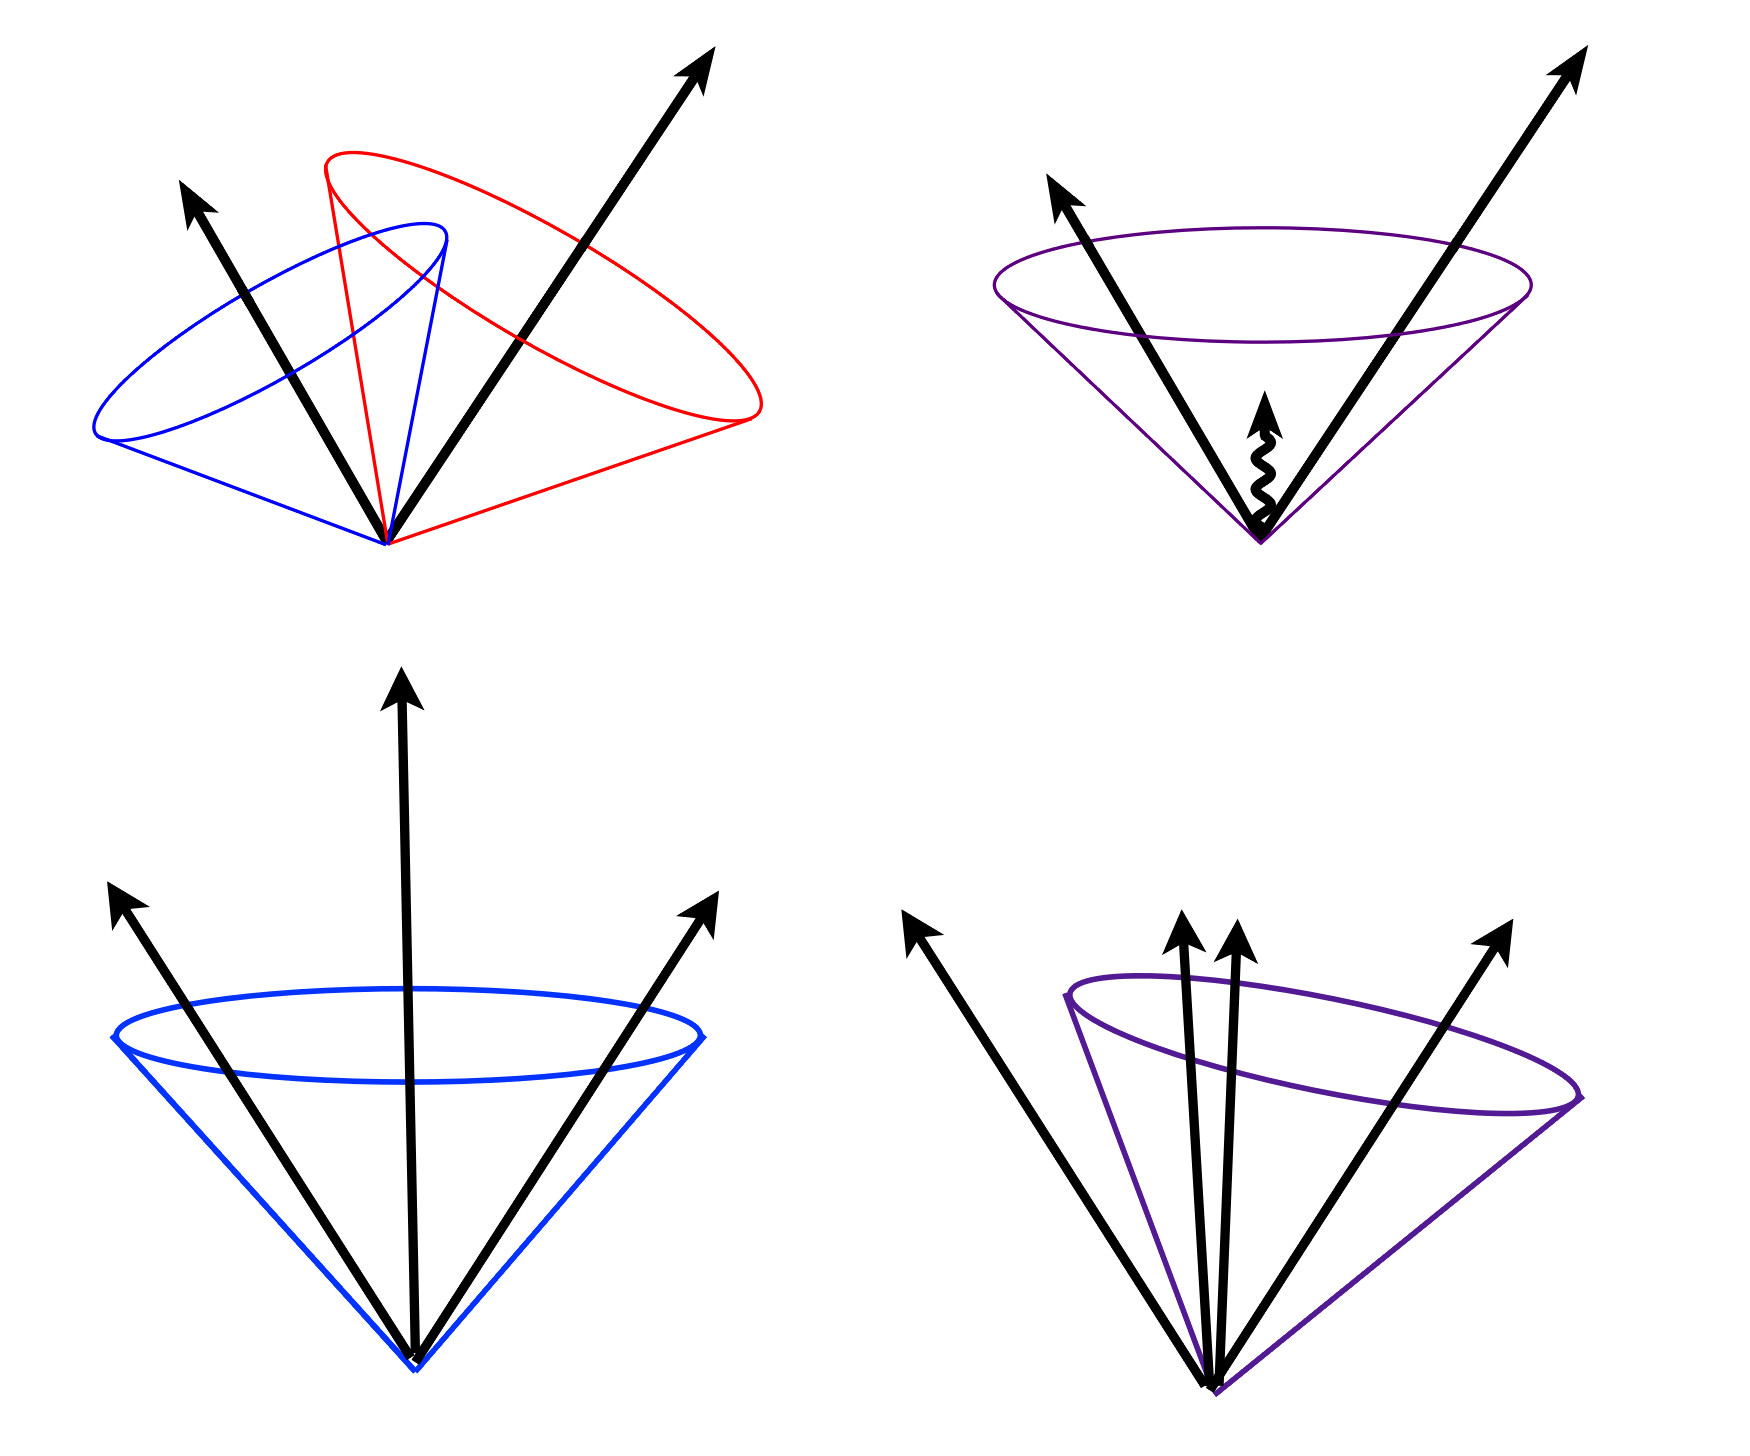
\includegraphics[width=0.7\columnwidth]{figures/Jets/IRCSafety.png}
%	\caption{Examples of the behavior of infrared and collinear unsafe jet algorithms.  In the top two diagrams, the addition of a soft gluon becomes the seed which a jet is centered on, causing the two jets to merge together into one jet.  In the bottom diagram, the splitting of the most energetic seed into two collinear ones, shifting the jet location and lowering the jet energy.  Diagram from \cite{IRCDiagram}.
%	}
%	\label{fig:IRCSafety}
%\end{figure}
%
%\subsection{The Anti-$k_t$ jet algorithm}
%A jet algorithm begins with a list of subjets, the individual inputs which will be combined to make jets.  In the case of ATLAS, the subjets are calorimeter topoclusters which are discussed in more detail in Section~\ref{sec:Topoclustering}, while for truth-level jets individual final state particles are used as subjets. The ATLAS jet definition of choice is the anti-$k_t$ algorithm.\cite{AntiKt} The anti-$k_t$ algorithm belongs to a family of sequential recombination algorithms which take the form:
%
%\begin{equation}
%	d_{ij} = \mbox{min}(k_{ti}^{2p},k_{tj}^{2p})\frac{\Delta_{ij}^2}{R^2}
%\end{equation}
%\begin{equation}
%d_{iB} = k_{ti}^{2p}
%\end{equation} 
%where $\Delta_{ij}^2 = (y_i - y_j)^2 + (\phi_i - \phi_j)^2$ is the distance between two subjets with rapidities $y_i$ and azimuths $\phi_i$, $k_{ti}$ is the transverse momentum of the subjet, and $R$ is the radius parameter which sets the size of the jet.  The parameter $p$ determines the behavior of the algorithm; $p=1$ corresponds to the $k_t$ algorithm~\cite{JetAlgos}, while $p=0$ gives the Cambridge/Aachen algorithm.\cite{CambridgeAachen}  Setting $p=-1$ gives the anti-$k_t$ algorithm.
%
%The algorithm begins by calculating $d_{iB}$ for each subjet and $d_{ij}$ for each pair of subjets, where the subjets are the input type to the algorithm.  The recombination proceeds from the smallest value of $d$.  If a $d_{ij}$ is smallest, the two subjets are combined, both their energy and their position, and all $d$ are recalculated using the new set of subjets.  If a $d_{iB}$ is smallest, the subjet is considered to be a full jet and is removed from the list of subjets.  An illustration of how this method proceeds is shown in Figure~\ref{fig:AKTExample}.
%
%\begin{figure}[]
%	\centering
%	\subfloat[]{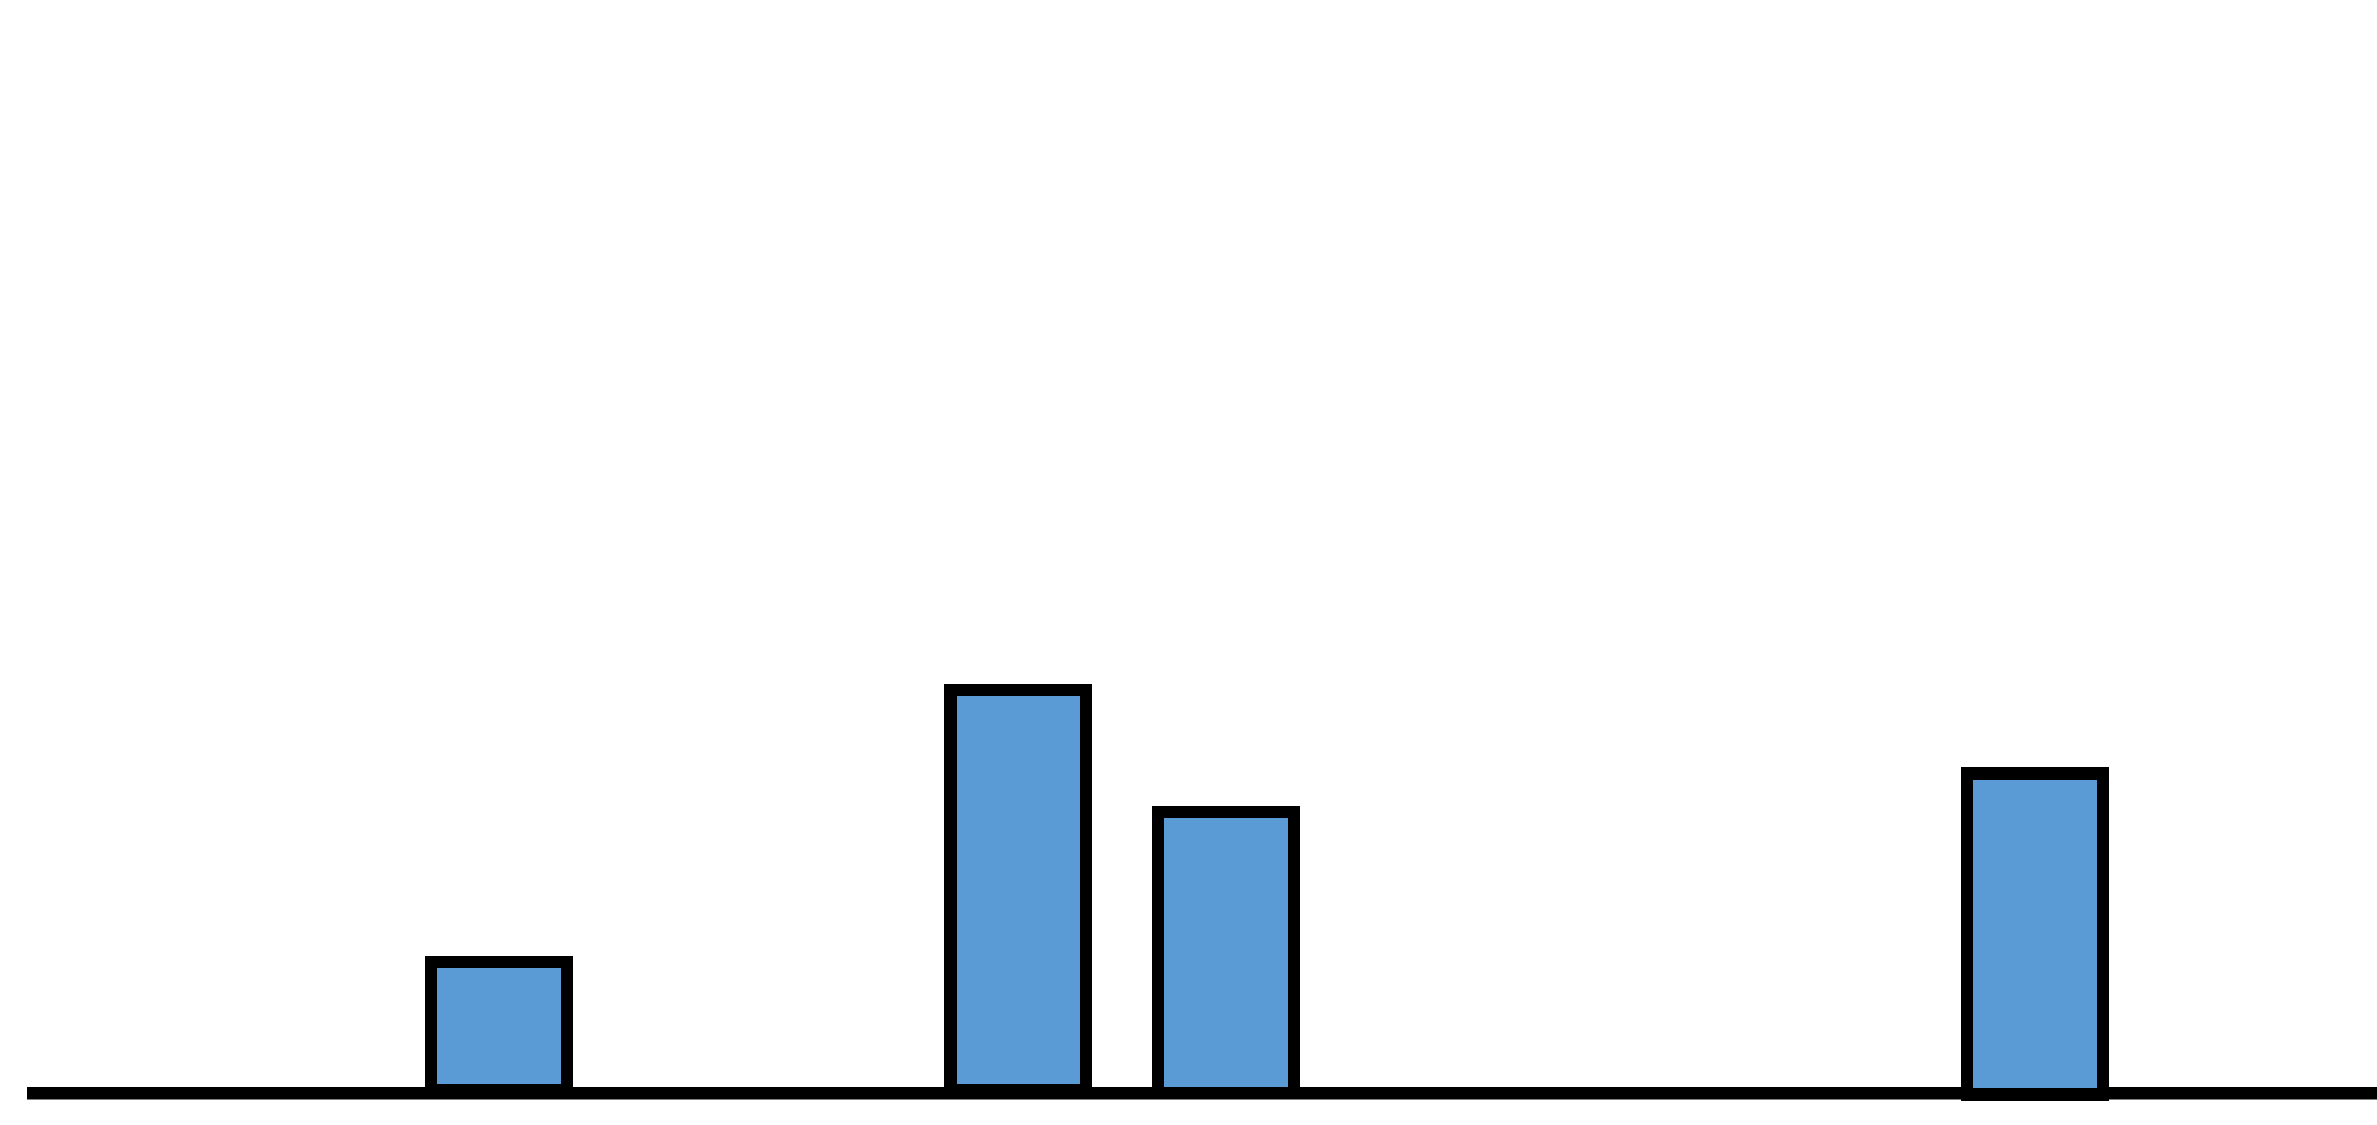
\includegraphics[width=0.45\columnwidth]{figures/Jets/AntiKt1.png}}
%	\hspace{0.1\columnwidth}%
%	\subfloat[]{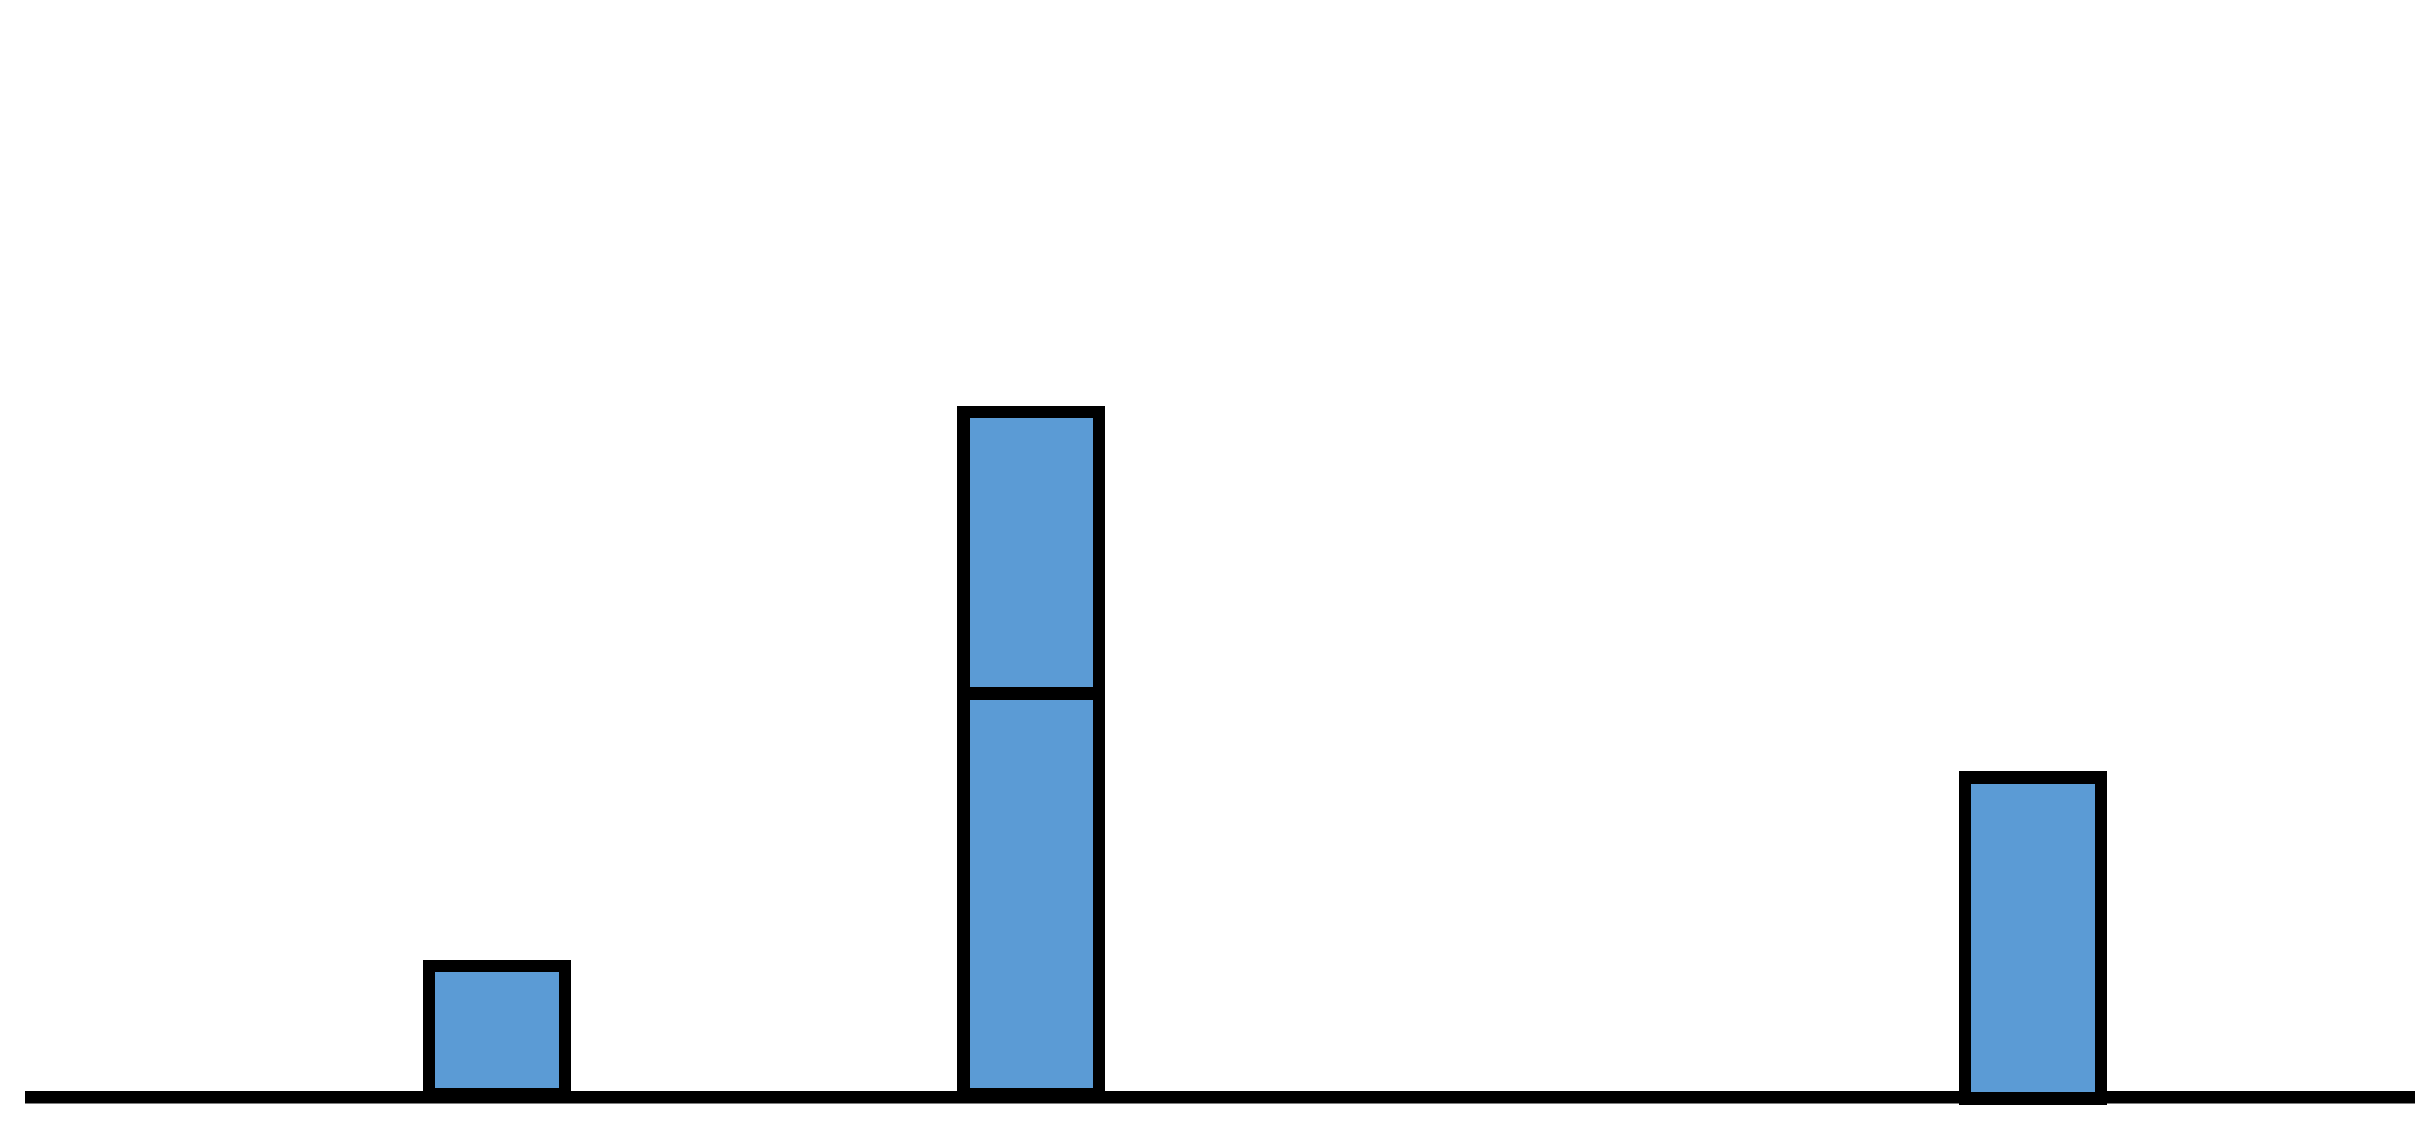
\includegraphics[width=0.45\columnwidth]{figures/Jets/AntiKt2.png}}
%	\hspace{0.1\columnwidth}%
%	\subfloat[]{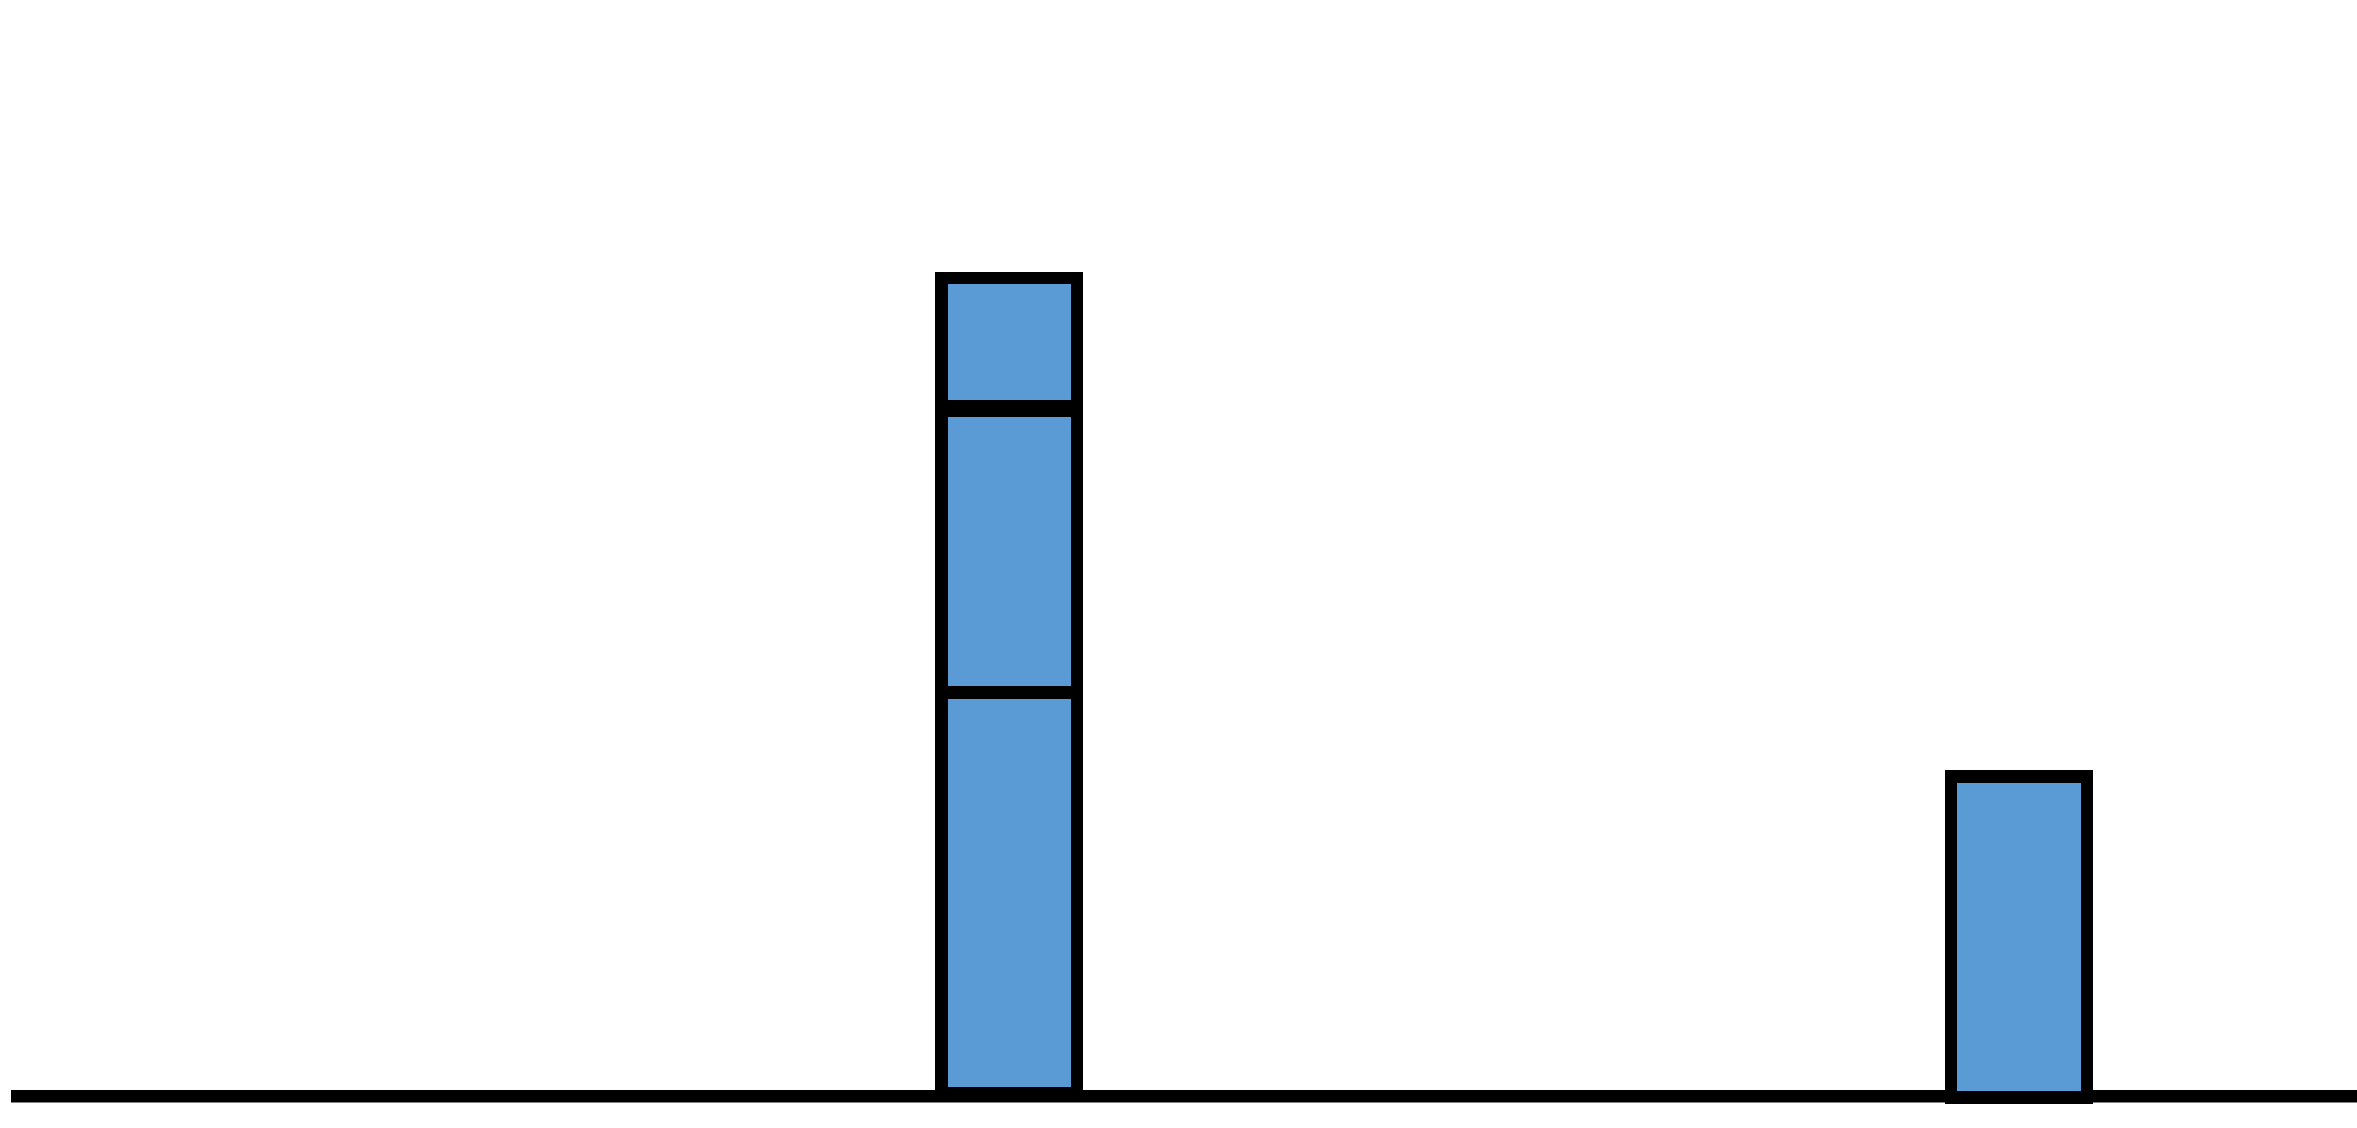
\includegraphics[width=0.45\columnwidth]{figures/Jets/AntiKt3.png}}
%	\hspace{0.1\columnwidth}%
%	\subfloat[]{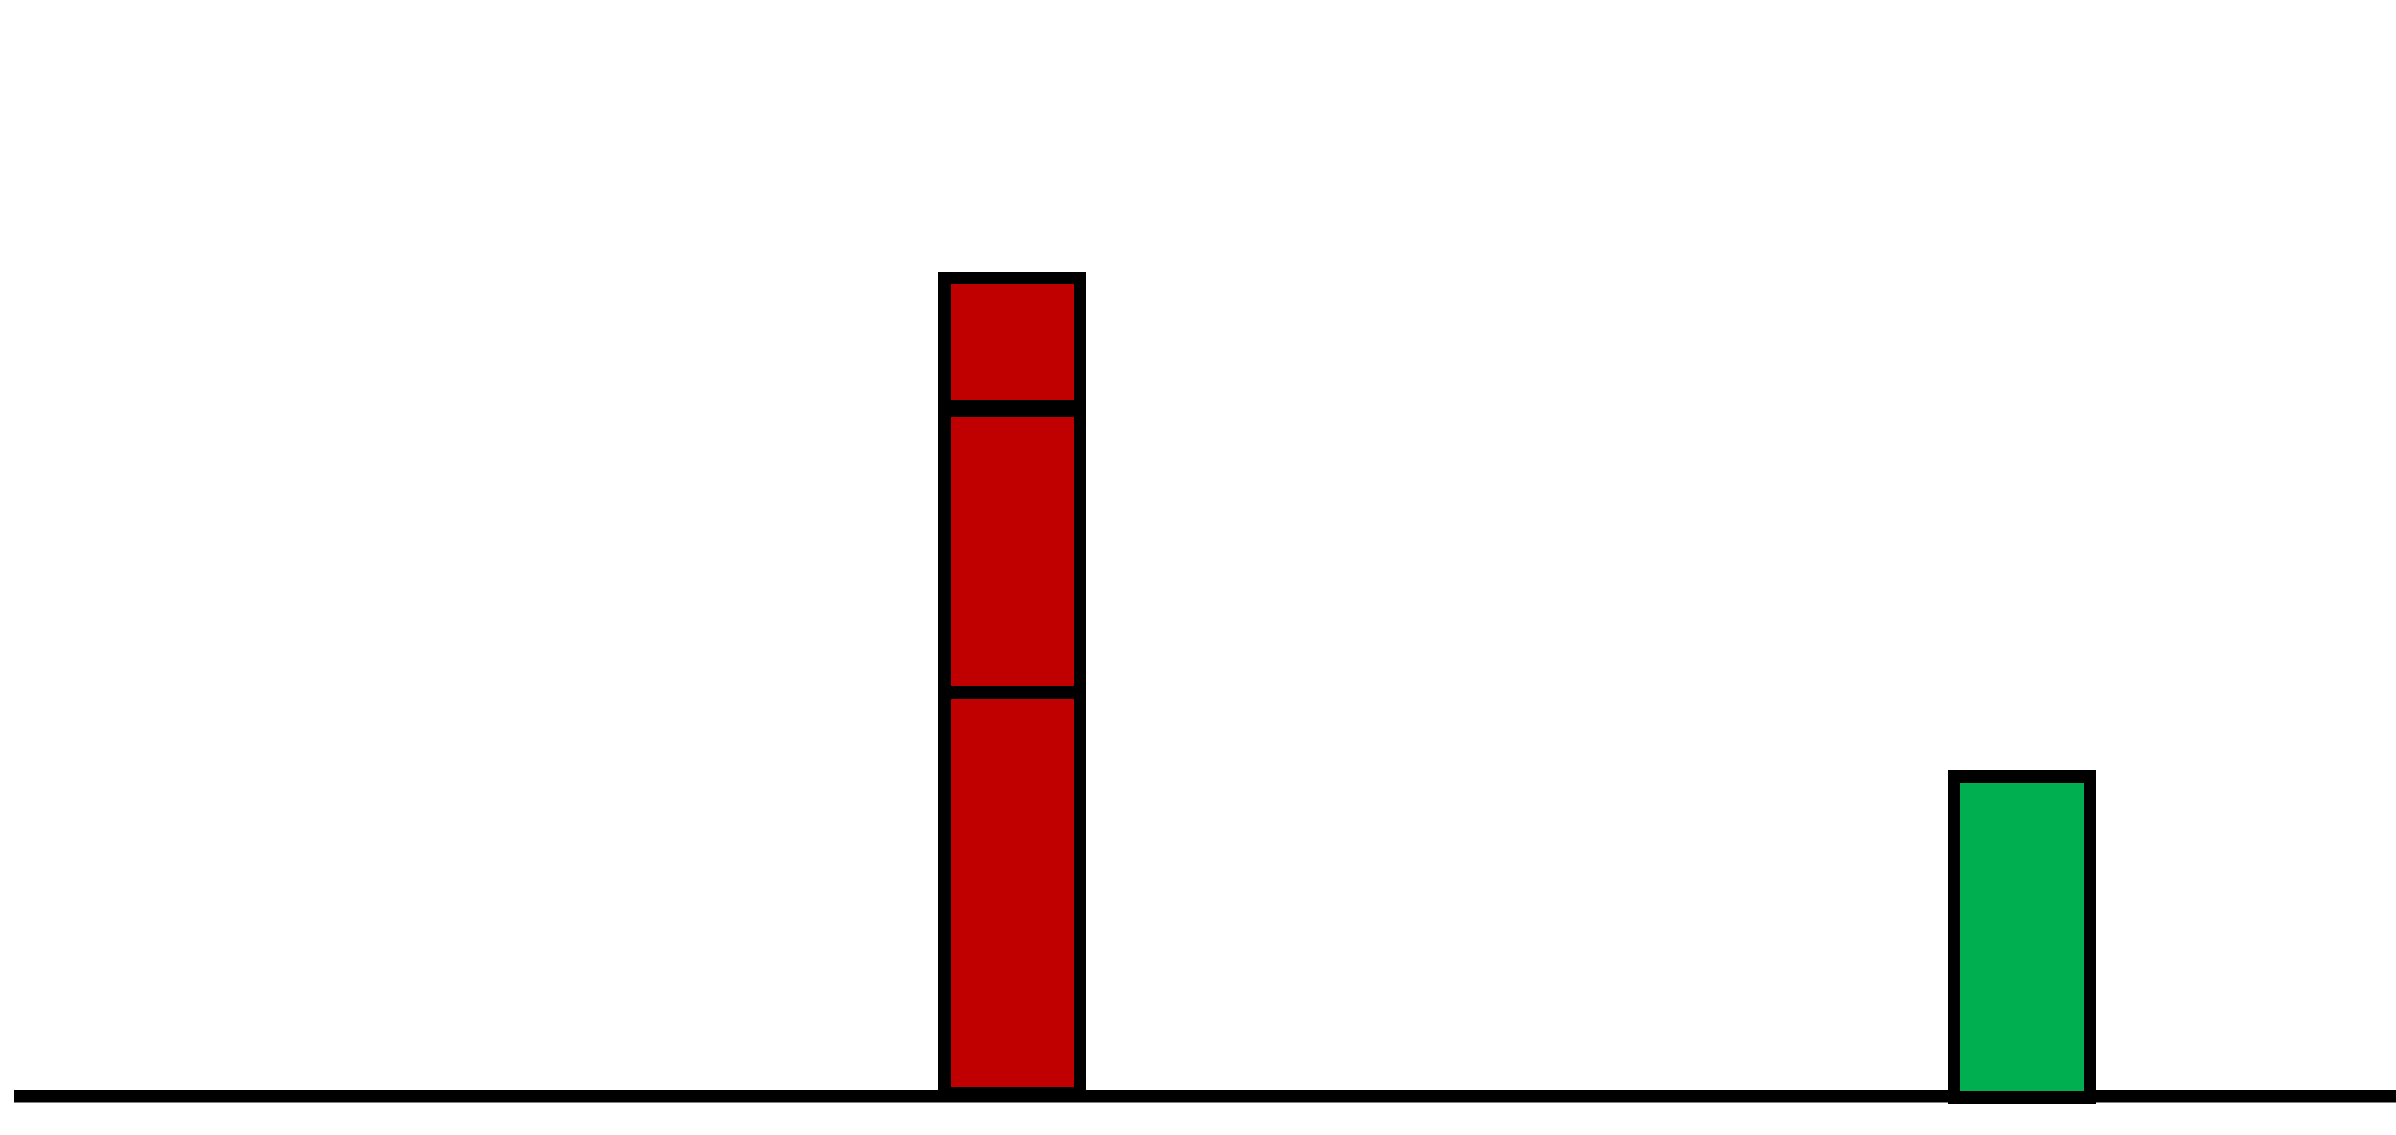
\includegraphics[width=0.45\columnwidth]{figures/Jets/AntiKt4.png}}
%	\caption{An example of the anti-$k_t$ recombination algorithm.  a) The original input subjets to the algorithm.  b) The highest \pt~subjet combines with its nearest neighbor to produce a new combined subjet.  c) This subjet again combines with its neighbor to produce a new subjet.  d) The remaining subjets are separated by more than the radius parameter of the algorithm.  The subjets become the final jets.}
%	\label{fig:AKTExample}
%\end{figure}
%
%The general behavior of the anti-$k_t$ algorithm is that the subjets with the highest transverse energy will cluster first, gathering together all of the smaller radiation around them, before the softer subjets begin clustering together.  The algorithm tends to produce roughly-conical jets, and gives preference to more energetic jets when two jets are close together.  An example of the final result of the anti-$k_t$ algorithm is shown in Figure~\ref{fig:AntiKtExample}.  Here, a single simulated event is shown along with thousands of very soft "ghost" particles which are randomly distributed and do not contribute any meaningful energy to the event.  These ghosts are used along with the real physics energy deposits in the jet algorithm but do not change the shape or location of the jets, allowing for the visualization and measure of the area encompassed by each jet.  This area is used to correct for the amount of pileup energy which falls within a jet.
%
%
%
%\begin{figure}[]
%	\centering
%	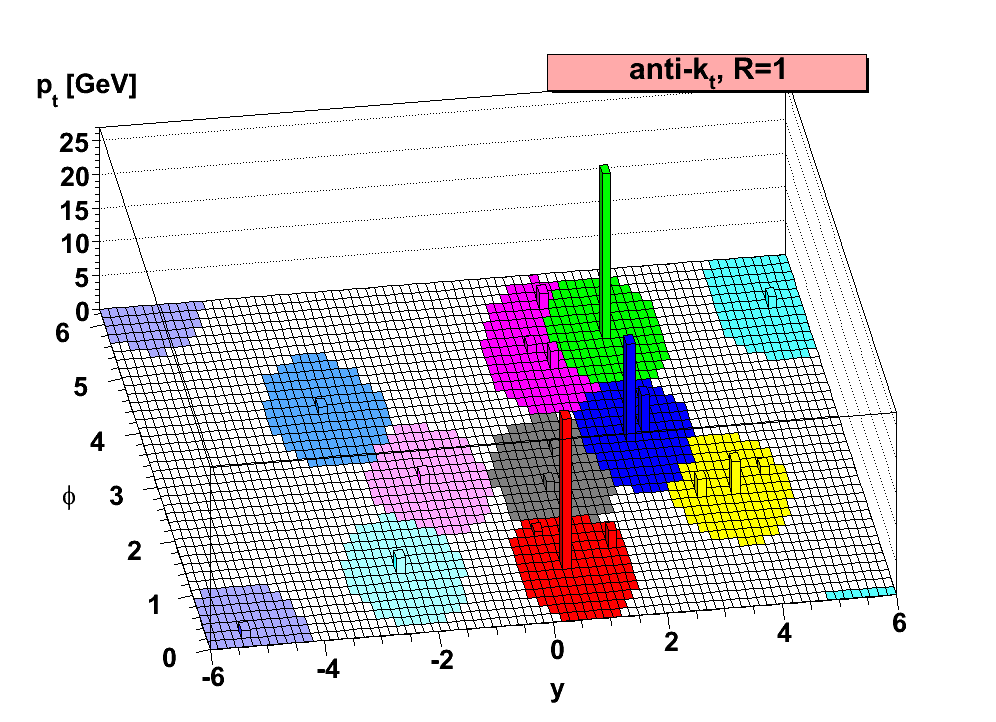
\includegraphics[width=0.7\columnwidth]{figures/Jets/AntiKtExample.png}
%	\caption{A sample parton-level event together with many random soft particles, clustered together using the anti-$k_t$ algorithm.\cite{AntiKt}.
%	}
%	\label{fig:AntiKtExample}
%\end{figure}
%
%As mentioned previously, the model of hadronization used to simulate the processes studied in this analysis has no meaningful impact on the sensitivity.  This is because the treatment of the hadronization step does not impact the location of the high-\pt~particles, but rather the distribution of soft emissions between them, and as such will have little impact on the \pt~as measured by the jet algorithm.
%
%The anti-$k_t$ algorithm is both collinear and infrared safe.  In the case of a collinear splitting of a hard particle into two softer ones, their small angular separation $\Delta_{ij}$ ensures that they will be clustered together at the beginning of the recombination, recovering the single hard particle.  The algorithm is infrared safe because a soft emission will first cluster to a highly energetic one and will not shift the jet, preventing any change in the final jet.  The choice of jet radius is somewhat arbitrary and depends on the physics process being investigated.  The standard ATLAS jet uses R=0.4, but other radii are used in specialized contexts such as R=0.2 jets to investigate jet substructure, and R=1.0 jets to capture the energy of boosted objects such a top quarks. 
